% cascade II /mnt/backup/safe-with-time/torben/safed/y2009/0414
% andor ultra ~/1114  python code for calibration and andor basic for acquisition
\chapter{Read noise characterization in cameras}
\label{sec:ccd-meas}
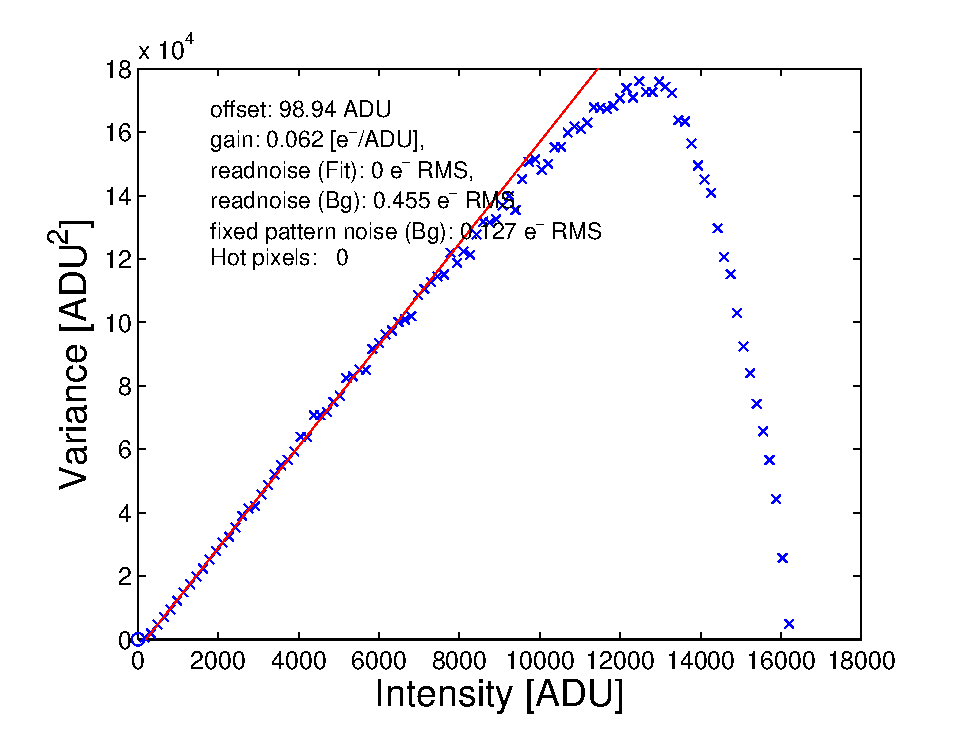
\includegraphics[width=8cm]{../app_cam/andor_emgain100_preamp5_exp30}
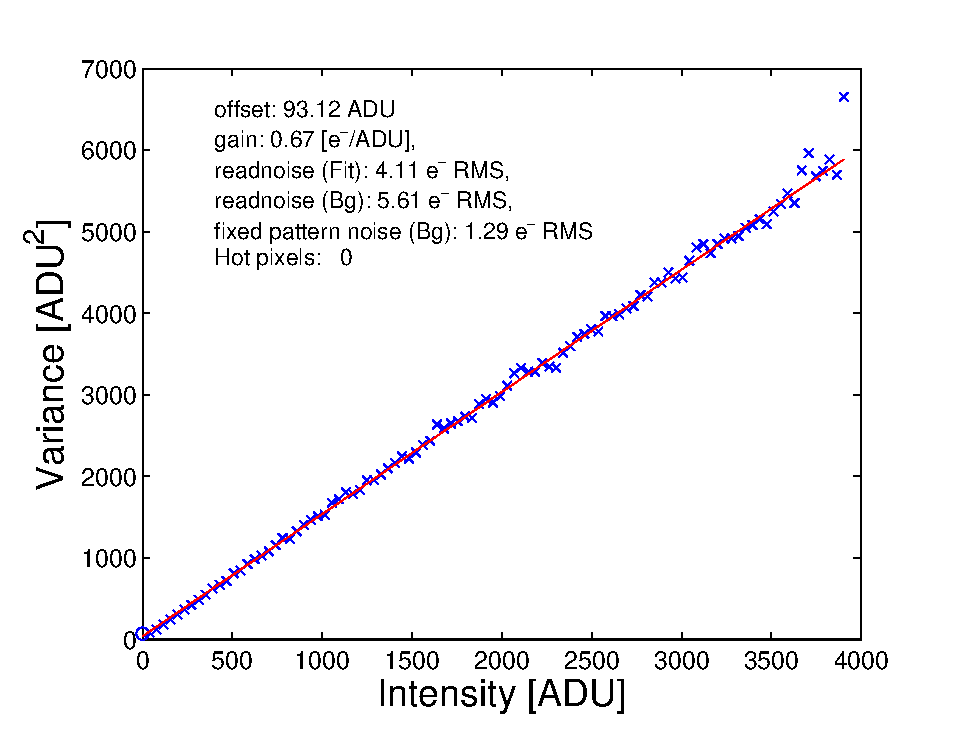
\includegraphics[width=8cm]{../app_cam/andor_normal_preamp5_exp30}
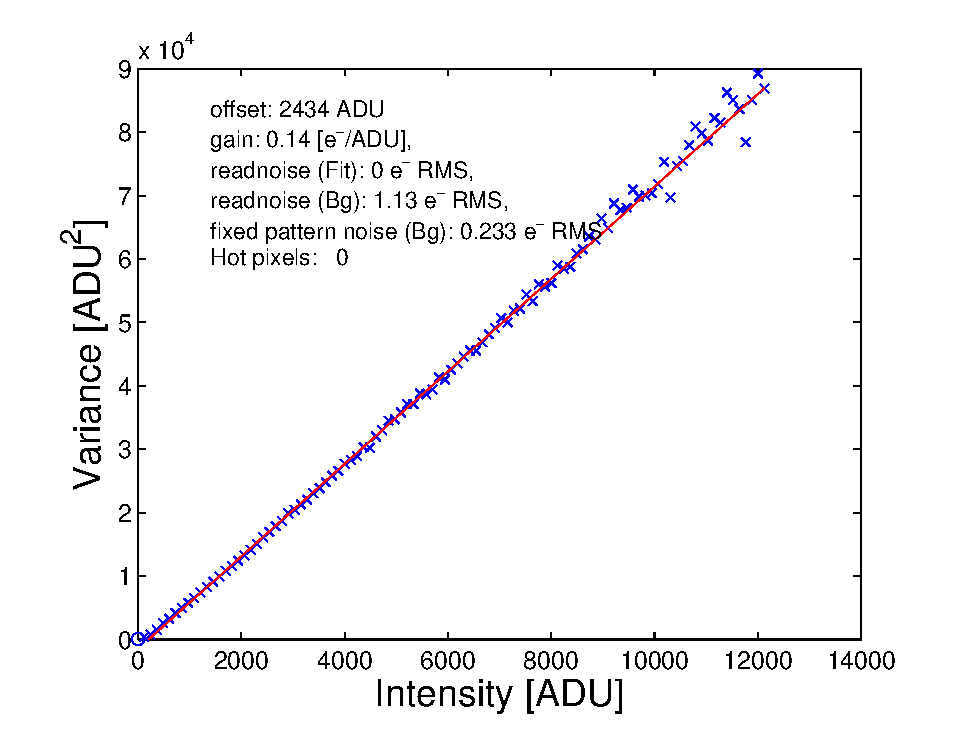
\includegraphics[width=8cm]{../app_cam/cascade_exp400ms_gain3000}
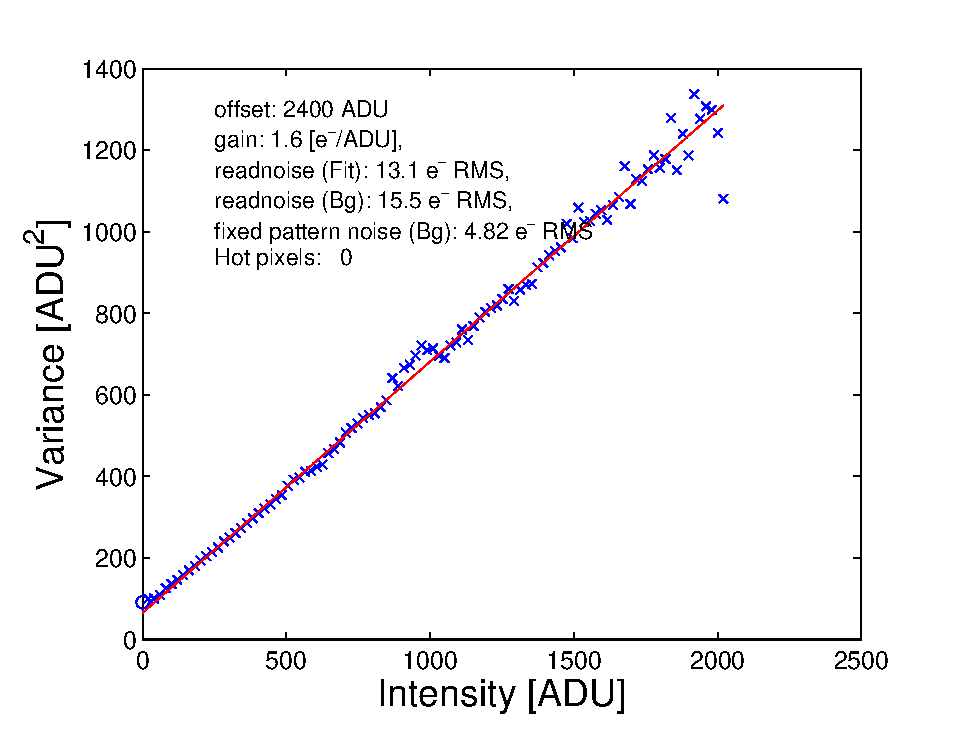
\includegraphics[width=8cm]{../app_cam/cascade_exp400ms_normal}
\includegraphics[width=8cm]{../app_cam/cascade_normal_preamp3_exp30}


\section{Introduction}
In order to characterize the camera we captured sequences of images
that contain a light pattern like this: \includegraphics[width=8cm]{calib-pic}

The images were produced in a fluorescence microscope. The light
source is a DPSS laser with \unit[473]{nm} wavelength. It illuminates
a circular area of the sample. The sample is a fluorescent plane. A
FITC filter cube and a $10\times$ objective were used. The sample was
adjusted to be slightly out of focus in order to obtain a smooth
intensity gradient in the image. For the comparison of the IXon3 with
the newer camera the sample wasn't changed. The Ultra was measured
first. The laser was mechanically blocked while the cameras were
swapped. The following figure depicts the intensity of 20 images that
were illuminated in this way. The relative standard deviation of the
illumination intensity was $0.15\%$.
%\includegraphics[height=7cm]{mean-light}

A sequence (e.g. 20) of such images can be used to determine the
mapping between arbitrary data units (ADU) and the number of detected
photoelectrons. This method is based on the known relation between the
mean number of Poisson distributed photons and its variance.

For the calibration a 2D histogram of the per pixel
variance image and the per pixel mean of the image stack is
plotted. Then the slope of the resulting point cloud is determined.
\section{Calibration of an older IXon3}

%\bbild{ixon_conv1}

In the left diagram of the figures above contains such a 2D
histogram. It was obtained for conventional readout at \unit[3]{MHz}
in our older IXon3 model. The variances are collected in 64 intensity
bins and their averages are plotted as red crosses. The blue line is
the result of a linear fit to the first $60\%$ of the red crosses. Its
slope gives the real gain of the camera that can be used to convert
ADU into photoelectrons (here \unit[1.32]{$e/$ADU}).

The following figures show corresponding measurements using the EM
readout mode with varying EM gain. It is followed by one last
measurement with conventional readout to verify, that the fluorophores
didn't bleach too much during the experiment.

For each figure 20 illuminated images and 20 dark images were
captured. The camera was cooled to \unit[$-75$]{$\,^{\circ}{\rm
    C}$}. The integration time was varied for each gain to have a
maximum of 10000 ADU using a short \unit[10]{ms} acquisition. This was
controlled by an Andor Solis Basic program.

The square root of the mean of the variance of the dark images was
converted into a read noise in electrons per pixel using the real
gain.

The exposure times for the various figures are given in the table that
follows below the figures.

\subsection{Source code for automatic image acquisition}
\begin{verbatim}
function ~GetSaturatingExposure()
        SetKineticNumber(1)
        exp=.01
        SetExposureTime(exp)
        run()
        m=maximum(#0,1,512)
        GetSaturatingExposure=exp*10000/(m-100)
        CloseWindow(#0)
return
name$ = "C:\Users\work\Desktop\martin\20111111\scan-em3\ixon_"
print("start")

SetOutputAmp(1)
print("conv_start")
exp= ~GetSaturatingExposure()
print(exp)
SetExposureTime(exp)
SetKineticNumber(20)
SetShutter(0,1)
run()
save(#0,name$ + "conv1_dark.sif")
ExportTiff(#0, name$ + "conv1_dark.tif", 1, 1, 0, 0)
CloseWindow(#0)
CloseWindow(#1)
        
SetShutter(1,1)
run()
save(#0,name$ + "conv1_bright.sif")
ExportTiff(#0, name$ + "conv1 _bright.tif", 1, 1, 0, 0)
CloseWindow(#0)
CloseWindow(#1)

SetOutputAmp(0)
SetShutter(1,1)
for i = 40 to 300 step 10
        SetGain(i)
        exp=~GetSaturatingExposure()
        print(exp)
        SetExposureTime(exp)
        SetKineticNumber(20)
        SetShutter(0,1)
        run()
        save(#0,name$ + str$(i) + "_dark.sif")
        ExportTiff(#0, name$ + str$(i) + "_dark.tif", 1, 1, 0, 0)
        CloseWindow(#0)
        CloseWindow(#1)
        SetShutter(1,1)
        run()
        save(#0,name$ + str$(i) + "_bright.sif")
        ExportTiff(#0, name$ + str$(i) + "_bright.tif", 1, 1, 0, 0)
        CloseWindow(#0)
        CloseWindow(#1)
next

SetOutputAmp(1)
print("conv_end")
exp= ~GetSaturatingExposure()
print(exp)
SetExposureTime(exp)
SetKineticNumber(20)
SetShutter(0,1)
run()
save(#0,name$ + "conv2_dark.sif")
ExportTiff(#0, name$ + "conv2_dark.tif", 1, 1, 0, 0)
CloseWindow(#0)
CloseWindow(#1)
        
SetShutter(1,1)
run()
save(#0,name$ + "conv2_bright.sif")
ExportTiff(#0, name$ + "conv2 _bright.tif", 1, 1, 0, 0)
CloseWindow(#0)
CloseWindow(#1)
\end{verbatim}

\subsection{Source code for the read noise evaluation}
\begin{verbatim}
#!/usr/bin/env python
# ./ti.py /media/backup/andor-ultra-ixon/martin/20111111/scan-em3/ ultra 2700
import sys
import os

import matplotlib
matplotlib.use('Agg')

from pylab import *
from libtiff import TIFFfile, TIFFimage
from scipy import stats

seterr(divide='ignore')

folder = sys.argv[1]
cam = sys.argv[2]
gain = sys.argv[3]


def readpics(gain,cam='ixon_',isdark=False):
    print 'loading ', os.path.join(folder,cam) + '_' + gain + '_bright.tif'
    fg=TIFFfile(os.path.join(folder,cam) + '_' + gain + '_bright.tif')
    bright,bright_names=fg.get_samples()
    bg=TIFFfile(os.path.join(folder,cam) + '_' + gain + '_dark.tif')    
    dark,dark_names=bg.get_samples()
    return (bright[0],dark[0])

(f,b) = readpics(gain=gain,cam=cam)

bg=mean(b,axis=0)
v=var(f,axis=0)
i=mean(f,axis=0)

ny,nx=64,128
H,y,x=histogram2d(v.flatten(),i.flatten(),bins=[ny,nx],
                  range=[[0,v.max()],[0,i.max()]])
extent = [x[0], x[-1], y[0], y[-1]] 
acc=zeros(x.shape,dtype=float64)
accn=zeros(x.shape,dtype=int64)
s=nx/i.max()
for ii,vv in nditer([i,v]):
    p=round(ii*s)
    acc[p]+=vv
    accn[p]+=1   


fig=figure(figsize=(24, 8),dpi=300)
#subplots_adjust(top=.7,bottom=.2)
hold(False)
title('bal')
subplot(1,3,1)
imshow(log(H), extent=extent,
           aspect='auto', interpolation='none',origin='lower')
hold(True)
ax=x[nonzero(accn)]
ay=acc/accn
ay=ay[nonzero(accn)]
l=round(.6*len(ax))
bx=ax[0:l]
by=ay[0:l]
plot(ax,ay,'r+')
slope,intercept,rval,pval,stderr=stats.linregress(bx,by)
plot(ax,polyval([slope,intercept],ax))
xlabel('intensity/ADU')
ylabel(r'variance/ADU$^2$')
real_gain=1/slope # unit electrons/ADU
read_noise=sqrt(var(b))*real_gain # electrons RMS per pixel
mean_elecs=(mean(f)-mean(b))*real_gain # photoelectrons electrons per pixel
print gain,cam,real_gain,read_noise,mean_elecs,mean(b),rval,pval,stderr
tit='EM-gain: %s, cam: %s, real gain: %.2f e/ADU\n
read noise: %.2f e RMS/pixel, mean: %.2f e/pixel, offset: %.2f'
% (gain,cam,real_gain,read_noise,mean_elecs,mean(b))
title(tit)
subplot(1,3,2)
imshow(var(b,axis=0))
title('variance of darkimages')
colorbar()
subplot(1,3,3)
imshow(mean(b,axis=0))
title('mean of darkimages')
colorbar()
show()
fig.savefig(cam+'_'+gain+'.png')
\end{verbatim}
